\documentclass{article}
\usepackage[utf8]{inputenc}
\usepackage{amsmath}


\title{Predicción del comportamiento de una enfermedad simulada en autómatas celulares con un algoritmo propuesto en redes neuronales}
\author{jibanezh }
\date{July 2021}

\usepackage{natbib}
\usepackage{graphicx}

\begin{document}

\maketitle

\section{Introducción}

\subsection{Epidemiología}

\subsubsection{¿Qué es la epidemiología?}
De acuerdo con \cite{epiDictionary}, la epidemiología se encarga de estudiar la ocurrencia y distribución de eventos, estados y procesos relacionados con la salud de distintas poblaciones, con el objetivo de brindar estrategias de control y prevención de problemas de salud relevantes.

\subsubsection{Breve historia de la epidemiología} 

El primer intento por modelar teóricamente la propagación de una enfermedad, fue realizado por Daniel Bernouilli en 1760, en el cual, basándose en sus conocimientos en medicina y matemáticas, desarrolló un modelo que describe el comportamiento de la viruela y evalúa el impacto teórico de la inoculación para su época \cite{shortHistory}. 

Sin embargo, en el modelamiento epidemiológico se considera como punto de partida el modelo descrito por Kermack y McKendrick en 1927, también conocido como modelo SIR, en el que se establecen relaciones entre tres estados de una enfermedad (Susceptible-Infectado-Recuperado) y se implementan los conceptos de tasa de contagio y de recuperación \cite{malariaSIR}. Desde entonces se han desarrollado múltiples variaciones sobre el modelo SIR, con el objetivo de analizar diferentes tipos de enfermedades de una manera más precisa, considerando por ejemplo diferentes estados, tasas de natalidad y mortalidad, entre otros \cite{diego2010}.

Por otra parte y debido a los avances tecnológicos de las últimas décadas, se han desarrollado modelos y simulaciones que permiten analizar características que no eran posibles con los modelos anteriormente mencionados. Por ejemplo, patrones de movilidad \cite{colaGNN, epidemiologicalNeuralNetwork}, disminución en la cantidad de contagios debido a un aislamiento preventivo \cite{stayHome}, contagios de individuo a individuo \cite{heterogeneousPopulation} e interacciones en masa \cite{combiningGraph, transfer2021}, la mayoría realizadas con una fuerte influencia de las redes neuronales y complejas, apoyadas fuertemente sobre la teoría de grafos.

\subsubsection{Modelos Compartimentales}

Tradicionalmente, se han utilizado modelos de compartimientos para elaborar análisis epidemiológicos. En estos modelos, cada individuo perteneciente a la población de estudio es clasificado en uno de $n$ posibles estados, según su estado de salud.

Las siglas de cada estado del modelo definen su nombre, por ejemplo, el modelo MSEIR define la interacción entre poblaciones con inmunidad "pasiva" o temporal (M), en donde la inmunidad de los individuos se genera a partir de los anticuerpos heredados de la madre. Con la desaparición de los anticuerpos, estos individuos se vuelven susceptibles a contraer la enfermedad (S). Si un individuo susceptible entra en contacto con un individuo infectado, pasará al estado de exposición (E) en donde ya se considera infectado pero incapaz de transmitir la enfermedad. En el momento en el que el individuo adquiera la capacidad de contagiar la enfermedad, se pasará al estado (I) y finalmente, cuando el individuo se recupere y adquiera inmunidad, pasará al estado (R) del modelo.\cite{modelCompartimental}

\begin{figure}[h.]
  \centering
    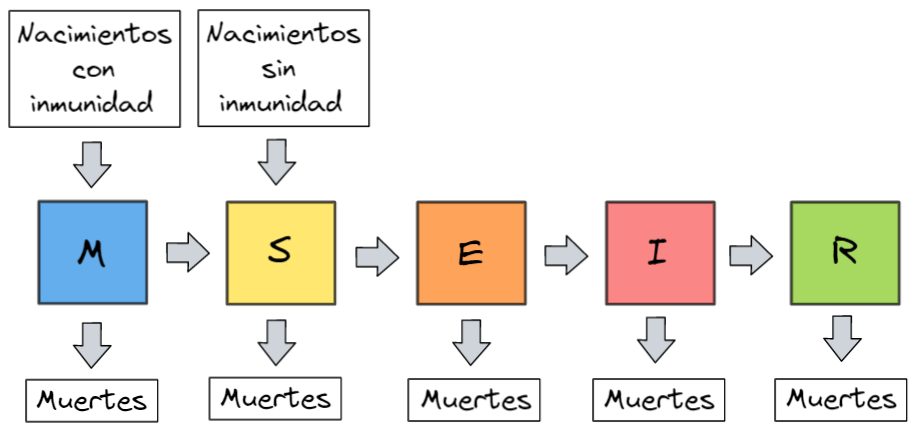
\includegraphics[width=0.8\textwidth]{Imagenes/MSEIR_compatimientos.PNG}
  \caption{Diagrama de compartimientos para el modelo MSEIR}
  \label{fig:ejemplo}
\end{figure}

\textbf{Nota:} Durante el desarrollo del presente documento trabajaremos con valores normalizados, por lo que 
$$\begin{array}{cc}
    M(t) + S(t) + E(t) + I(t) + R(t) = 1 & \text{, para todo tiempo }t.
\end{array} $$

\subsubsection{Estudio epidemiológico}
Uno de los objetos de estudio con mayor importancia en el campo de la epidemiología es la cualidad endémica de la enfermedad, es decir, si la enfermedad afectará a la población por un largo periodo de tiempo o si desaparecerá gradualmente. La manera en la que se determina está capacidad está dada por los siguientes indicadores:

\begin{itemize}
    \item \textbf{Número básico de reproducción $R_0$:} Se define como la cantidad de individuos que infecta el paciente cero en una población completamente susceptible. En general, si $R_0<1$ la enfermedad desaparecerá paulatinamente y sí $R_0>1$, podríamos estar ante un caso de endemia.
    \item \textbf{Número de contactos adecuados $\sigma(t)$:} Es la cantidad de contactos con individuos del sistema que realiza un individuo infectado durante su etapa de infección, cuando se introduce en la población en el momento $t$.
    \item \textbf{Número de desplazamiento $R(t)$:} Se entiende como la cantidad promedio de infecciones secundarias que produce un individuo infectado durante su etapa de infección, cuando es introducido en la población en el momento $t$. De ese modo, $R(t) = \sigma(t)\cdot S(t)$, donde $S(t)$ indica la cantidad de individuos susceptibles en el momento $t$.
\end{itemize}

\subsubsection{Función de supervivencia}
Heesterbeek y Dietz definen el número básico de reproducción $R_0$ como
\begin{equation}
    R_0 = \int_0^\infty b(a)F(a) da
\end{equation}
donde $b(a)$ representa la cantidad promedio de nuevos contagios que producirá un individuo infectado durante un tiempo y $F(a)$, conocida como la función de supervivencia, representa la probabilidad de que un individuo recién infectado se mantenga en ese estado durante al menos un tiempo $a$ \cite{conceptOfR0, perspectivesOnR0}.

\subsection{Modelos SIS y SIR determinísticos}
\subsubsection{Modelo SIS}


\section{Marco teórico}

\subsection{Modelo sis}
\begin{itemize}
    \item planteamiento del modelo sis 
    \item explicación del método de Euler 
    \item pseudo codigo de la implementación
    \item solucion del modelo 
    \item analisis de metricas descritas en la subseccion anterior
\end{itemize}
\subsection{Modelo sir}
\begin{itemize}
    \item planteamiento del modelo sir
    \item solucion del modelo 
    \item analisis de metricas descritas en la subseccion anterior
\end{itemize}

\bibliographystyle{plain}
\bibliography{references}
\end{document}